\section{Production Frontier}

We define the production frontier as the set of points which can not be
achieved by producing a different vector and then throwing away things:
\[
	\pf(X) := \{ x\in X : \nexists y\in X \text{ with } x\prec y\}
\]
where \(x\prec y\) is defined to be \(x^{(i)} \le y^{(i)}\) for all \(i\) and
there exists at least one \(i\) where the inequality is strict.

\begin{lemma}[Production Frontier is part of the Boundary of X]
	\label{lem: prod frontier part of boundary}
	\[
		\pf(X)\subseteq \partial X
	\]
\end{lemma}
\begin{proof}
	For any \(x=(x^{(1)},\dots, x^{(\dims)})\in X^\circ\) exists \(\epsilon>0\)
	such that \(x_{+\epsilon} = (x^{(1)}+\epsilon, \dots, x^{(\dims)}+\epsilon)\)
	is an element of \(X\). But then \(x\) can not be an element of \(\pf(X)\),
	since \(x \prec x_{+\epsilon}\).
\end{proof}

To characterize the production frontier further, we are going to assume
convexity of \(X\). We have motivated the asymptotic convexity of the
average production capabilities \(\bar{X}_n\) in Lemma~\ref{lem: clone prod
cap}. While this asymptotic convexity does not translate to convexity of \(X\)
one could easily replace \(X\) with \(\bar{X}_n\) in the following, at the
expense of notational simplicity.

\begin{lemma}[Duality of Support Function]
	\label{lem: duality of support function}
	If \(X\) is a compact, convex \ref{eq: lower
	layer}, then for any \(x\in \partial X\), there exists
	\(p\neq 0\) such that
	\begin{equation}
		\label{eq: prod frontier p}
		x \in \argmax_{y\in X} \langle p, y\rangle %= \nabla_p \mu(p, X)
	\end{equation}
	and therefore
	\[
		\mu(p, X) = \langle p, x\rangle.
	\]
	If additionally \(x\in\real_{>0}^\dims\), then necessarily \(p\in\real_{\ge
	0}^\dims\) if \(p\) satisfies \eqref{eq: prod frontier p}.
\end{lemma}
\begin{proof}
	Let \(x\in \partial X\), define \(A:=X^\circ\) and \(B:=\{x\}\). Then \(A\)
	is open; \(A\) and \(B\) are disjoint, nonempty
	convex subsets of \(\real^\dims\). So by the hyperplane separation theorem
	there exists
	\(0\neq p\in\real^\dims\) and \(c\in\real\) with
	\[
		\forall y\in A : \langle y, p\rangle < c
		\qquad\text{and}\qquad
		\langle x, p\rangle \ge c.
	\]
	Due to continuity of the scalar product we also have \(\langle y, p\rangle
	\le c\) for all \(y\in X\). Since \(x\in X\) this implies
	\begin{equation}
		\label{eq: x is max w.r.t. p}
		\langle y, p\rangle \le c = \langle x, p\rangle \quad \forall y\in X
	\end{equation}
	Therefore \(x\in\argmax_{y\in X} \langle p, y\rangle\) and \(\mu(p, X) =
	\langle x, p\rangle\).

	Let us now consider \(x=(x^{(1)},\dots,x^{(\dims)})\in\real_{>0}^\dims\).
	To arrive at a contradiction, we assume \(p_i < 0\). Since \(x^{(i)}>0\) and
	\(X\) is a \ref{eq: lower layer}, we can replace the entry \(x^{(i)}\) with
	\(0\) to obtain \(\tilde{x}\in X\). Then
	\[
		\langle \tilde{x}, p\rangle
		= \sum_{\substack{j=1\\i\neq j}} x^{(j)} p_j
		> \underbrace{x^{(i)}}_{>0}\underbrace{p_i}_{<0}
		+ \sum_{\substack{j=1\\i\neq j}} x^{(j)} p_j
		= \langle x, p\rangle,
	\]
	which is a contradiction to \eqref{eq: x is max w.r.t. p}.
\end{proof}

\begin{theorem}[Production Frontier Characterization]
	If \(X\) is a compact, convex \ref{eq: lower layer}, then
	\[
		\bigcup_{p\in \real_{>0}^\dims} \argmax_{y\in X}\langle p, y\rangle
		\subseteq \pf(X) \subseteq
		\bigcup_{p\in \real_{\ge 0}^\dims\setminus\{0\}}
		\argmax_{y\in X}\langle p, y\rangle.
	\]
	Where the first subset property does not actually require any restrictions on
	\(X\). Its interpretation is, that any maximization with regards to positive
	prices will result in a point on the production frontier.

	The second subset property can be interpreted as: For any point \(x\) on the
	production frontier, there exist non-negative prices \(p\) such that
	maximization with regards to \(p\) leads to production of \(x\).
\end{theorem}
\begin{proof}
	For any \(p\in\real_{>0}^\dims\) we have
	\[
		\argmax_{y\in X}\langle p, y\rangle \subseteq \pf(X).
	\]
	Because if we take any \(x\) from the first
	set, and assume there would exist \(x_+\in X\) with \(x\prec x_+\), then we
	would have \(\langle x, p\rangle < \langle x_+, p\rangle\) following from
	\(p\in \real_{>0}^\dims\). But that is a contradiction. Therefore
	\(x\in\pf(X)\). Taking the union over all such \(p\) implies
	\[
		\bigcup_{p\in \real_{>0}^\dims} \argmax_{y\in X}\langle p, y\rangle \subseteq \pf(X).
	\]

	Now let \(x\in \pf(X)\). If \(0\in\pf(X)\), then \(X=\{0\}\). So without loss
	of generality let \(x\neq 0\) and \(I\) be the set of indices \(i\) where
	\(x^{(i)}\neq 0\). We now consider the subspace
	\[
		\real^I := \{y\in \real^\dims : y^{(i)} = 0, \quad \forall i \in I^\complement\}
	\]
	which can be identified with \(\real^{|I|}\). \(X\cap\real^I\) is a compact,
	convex \ref{eq: lower layer} again and it is straightforward to verify
	\[
		x\in \pf(X)\cap \real^I
		\subseteq \pf(X\cap \real^I)
		\overset{\text{Lem.~\ref{lem: prod frontier part of boundary}}}\subseteq
		\partial(X\cap\real^I).
	\]
	So by Lemma~\ref{lem: duality of support function} there exists \(p\in
	\real^I\setminus \{0\}\), such that 
	\begin{equation}
		\label{eq: x is optimal w.r.t. p on subspace}
		x\in \argmax_{y\in X\cap\real^I} \langle p, y\rangle.
	\end{equation}
	And as \(x\in\real_{>0}^I\) by definition of \(I\), we have \(0\neq
	p\in\real_{\ge 0}^I\). Interpreting \(p\) as a member of \(\real_{\ge
	0}^\dims\) again, we can finish this proof if we can show that for this \(p\)
	\[
		x\in\argmax_{y\in X}\langle p, y\rangle.
	\]
	Assume that this were not the case. Then there would exist \(x_+\in X\)
	such that
	\[
		\sum_{i\in I}p_i x^{(i)}
		= \langle p, x\rangle
		< \langle p, x_+\rangle
		\overset{p\in\real^I}= \sum_{i\in I} p_i x_+^{(i)}
	\]
	As the \(x^{(i)}_+\) for \(i\notin I\) do not contribute to the scalar product,
	we can w.l.o.g. replace them with \(0\) due to the lower layer property.
	But then \(x_+\in X\cap \real^I\), which is a contradiction to \eqref{eq: x
	is optimal w.r.t. p on subspace}.
\end{proof}



\begin{figure}
	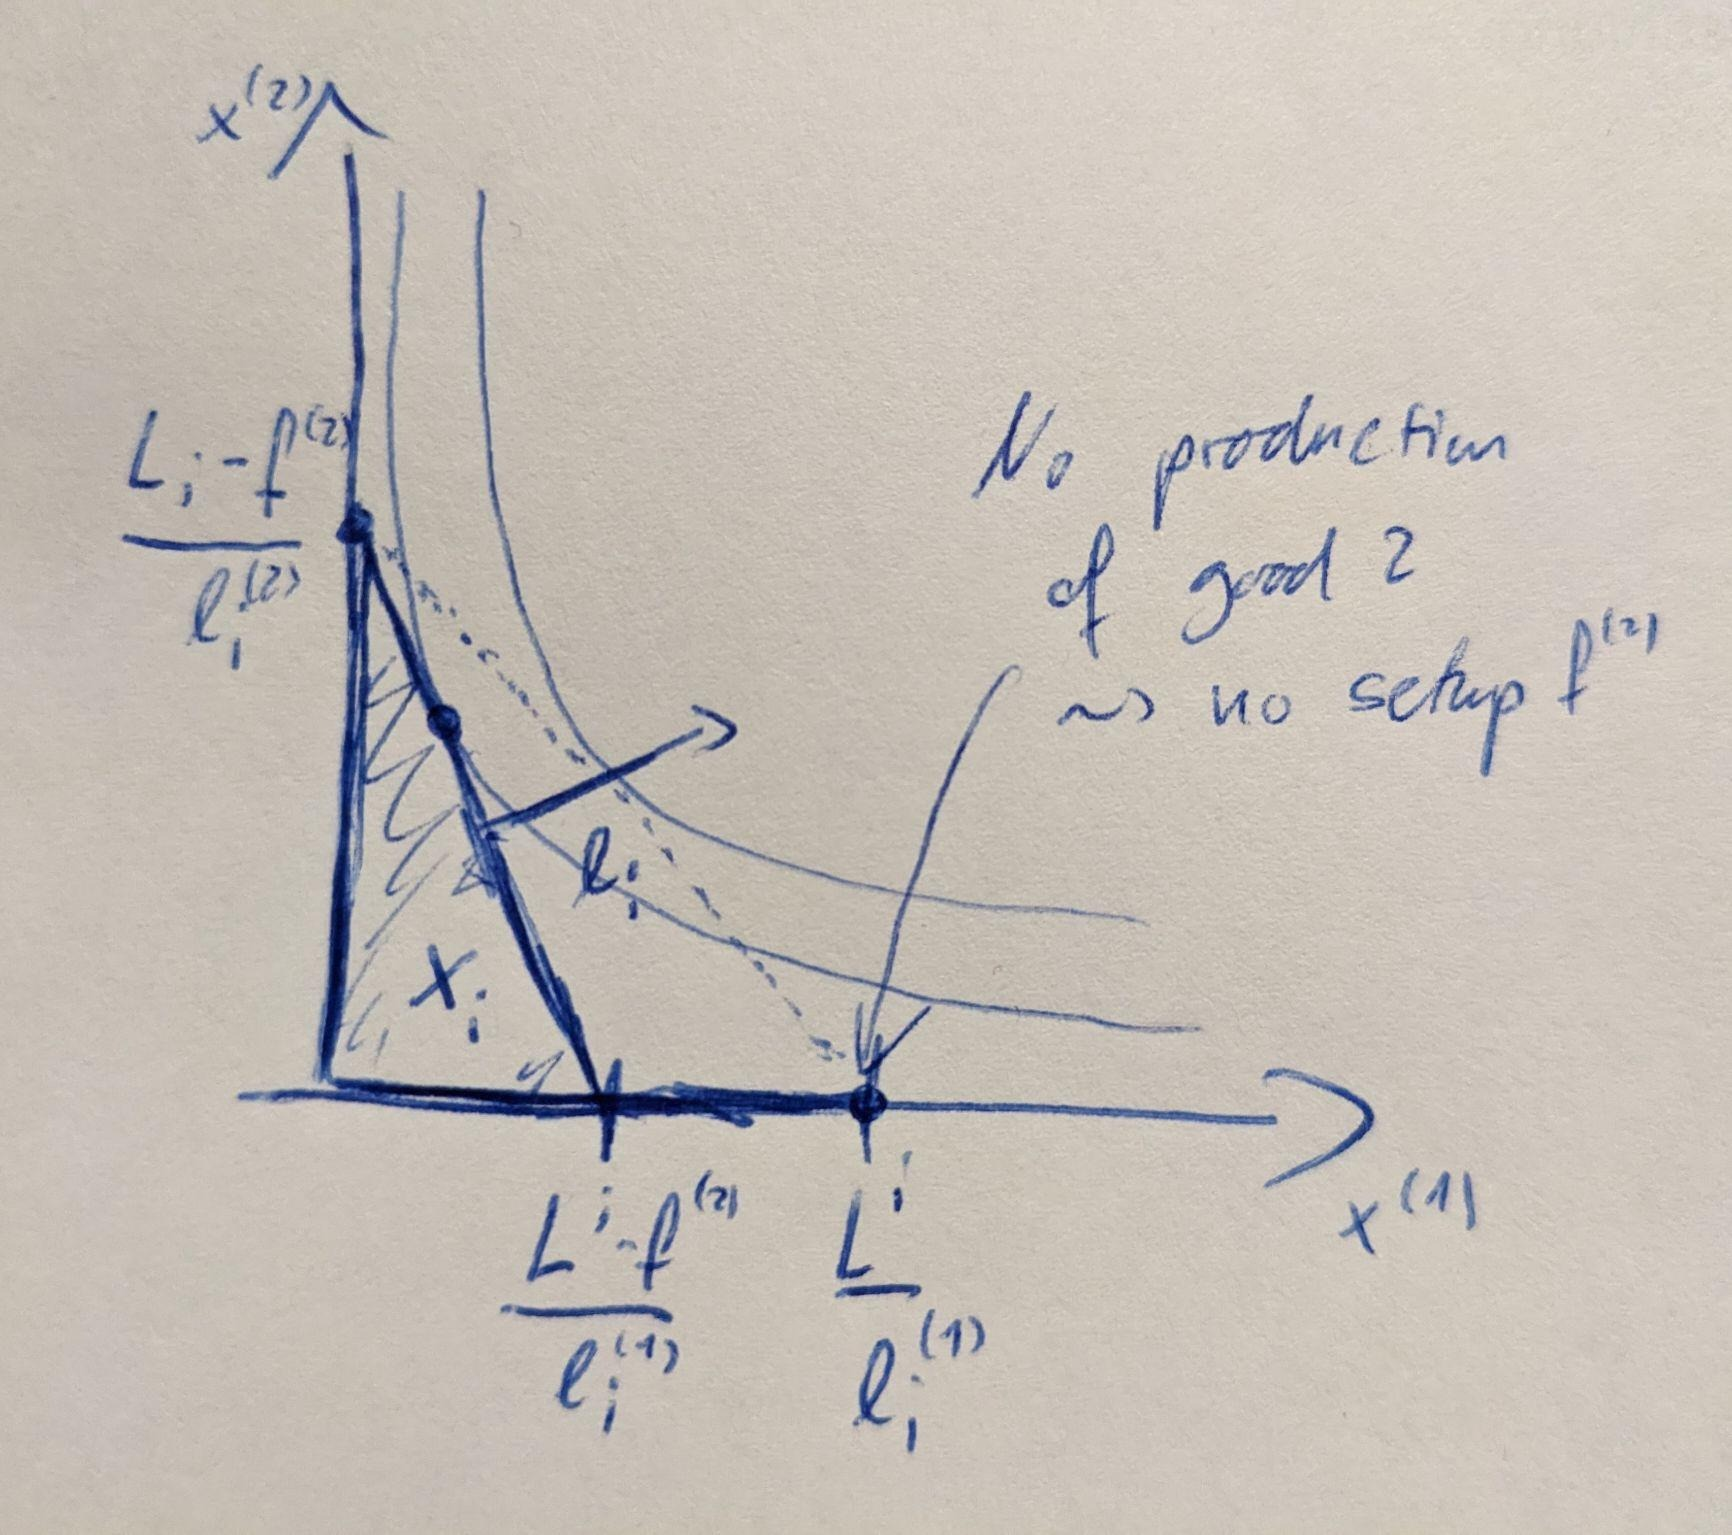
\includegraphics[width=0.58\textwidth]{images/hermit-decision-setup-cost.jpeg}
	\caption{
	fixed set-up time \(f^{(2)}\) for the production of good \(2\). This allows
	for more production of good \(1\) if \(x^{(2)}=0\). The dotted line
	represents the production frontier in the ``cloned hermit economy''.}
\end{figure}